\documentclass[a4paper,12pt]{article}

\usepackage[left=2.5cm,top=2.5cm,right=2.5cm,bottom=2.5cm]{geometry}

\usepackage[T1]{fontenc}
\usepackage[spanish]{babel}
\usepackage[utf8]{inputenc}

\usepackage[pdftex, breaklinks=false, colorlinks=true, linkcolor=black, anchorcolor=black, urlcolor=blue, citecolor=red]{hyperref}

%\usepackage{framed}

% \usepackage{amsfonts}
% \usepackage{amssymb}
% \usepackage{amsthm}
% \usepackage{amsmath}
% \usepackage{array}
% \usepackage{caption}
% \usepackage{color}
% \usepackage[mirror]{crop} %<--------------LOL
% \usepackage{eurosym} %para el simbolo del euro
% \usepackage{fancybox}
% \usepackage[Rejne]{fncychap}% Sonny, Glenn, Lenny, Conny, Rejne, Bjarne
% \usepackage{float}
% \usepackage{fullpage}
% \usepackage{graphicx}
% \usepackage{multirow}
% \usepackage{pifont}
% \usepackage{stmaryrd}
% \usepackage{supertabular}
% \usepackage[dotinlabels]{titletoc}
% \usepackage[all]{xy}
% \usepackage{wasysym}




%\usepackage{tikz}
\usepackage{times}

%\usepackage{xxcolor}

%\usepackage{mathdesign}
%\usepackage{titlesec}


%\usepackage{estiloBase}
%\usepackage{colores}
%\usepackage{bera}
\usepackage{comandos}

% \usepackage{setspace}

% \usepackage{calc}

% \addto\captionsspanish{
% \renewcommand\bibname{Bibliografía y referencias}
% }

\def \titulo{SiteUp: plataforma para la vigilancia de la disponibilidad de servicios de Internet}
\def \autor{Alumno: José Tomás Tocino García\\Tutores: Iván Ruiz Rube}
\def \fecha{Mayo de 2014}

% Directorio de imágenes
%\graphicspath{{../img/}}

\usepackage{parskip}
\usepackage{abstract}

\begin{document}
\portada

\vspace{0.25cm}

\begin{abstract}
\textbf{SiteUp} es un proyecto para la vigilancia de la disponibilidad
  de servicios de Internet. Consta de una plataforma web, en la que los usuarios
  tienen la posibilidad dar de alta chequeos de varios tipos: envío de pings,
  chequeo de puertos, chequeo de registros DNS y comprobaciones mediante
  peticiones HTTP. Estos chequeos son ejecutados por el sistema de forma
  periódica y generan notificaciones cuando detectan fallos. Estas
  notificaciones se envían mediante correo electrónico o a través de SiteUp
  Client, una aplicación Android desarrollada a tal efecto. Los usuarios tienen
  también la posibilidad de revisar la información obtenida de los chequeos a
  través de la web a lo largo del tiempo. \\

  \textbf{Palabras clave:} Internet, Web, Servicio, SaaS, Vigilancia,
  Disponibilidad, Monitorización

\end{abstract}


\vspace{0.5cm}

\begin{center}
{\footnotesize Este documento se halla bajo la licencia FDL de GNU (Free Documentation
  License)\\ \url{http://www.gnu.org/licenses/fdl.html} }   
\end{center}



\tableofcontents

\section{Introducción}

\subsection{Contexto y motivación}

Las tecnologías de la información en general e Internet en particular son ya
parte integral de la sociedad. Casi todos los ámbitos de la vida, desde las
interacciones sociales hasta la búsqueda de empleo, cuentan ya con su reflejo en
las tecnologías de la información. Además, han surgido nuevos modelos
empresariales propios de Internet que han crecido a niveles comparables a los de
los negocios tradicionales. Empresas puramente digitales como Facebook o Twitter
ya cotizan en bolsa y realizan operaciones bursátiles del orden de miles de
millones de dólares~\cite{facebook-acquires-whatsapp}.

Se pone así de manifiesto la importancia de la fiablidad de los servicios e
infraestructuras de los que dependen estos nuevos modelos de negocio. La
disponibilidad debe ser siempre cercana al 100\%, dado que en caso contrario los
potenciales usuarios del servicio se encontrarán con que no pueden acceder a él,
dando lugar incluso a pérdidas económicas. Es el caso de Amazon, que llegó a
perder 4.8 millones de dólares al sufrir un fallo que dejó inaccesible su web
durante 40 minutos~\cite{amazon}.

\textbf{SiteUp} se modela como una herramienta de monitorización de servicios de
Internet accesible a través de la web. Los usuarios tendrán la posibilidad de
crear y gestionar una serie de \textit{chequeos} de diversos tipos sobre los
servicios web que elijan. La aplicación irá recopilando información relativa a
esos chequeos, e informará al usuario en caso de que las verificaciones que se
hayan dado de alta no coincidan con los resultados esperados.

Además, el usuario tendrá la posibilidad de recibir notificaciones de manera
instantánea a través del correo electrónico y de una aplicación para la
plataforma móvil \textbf{Android}. 


\subsection{Objetivos}
Los principales objetivos a alcanzar con \textbf{SiteUp} son los siguientes:

\begin{itemize}

\item Crear un conjunto de herramientas para la monitorización y el chequeo de
  diversos aspectos del estado de un servicio de Internet.
\item Crear una aplicación online, de acceso público, que permita la creación y
  gestión de chequeos de manera sencilla, basada internamente en las
  herramientas mencionadas en el punto anterior.
\item Habilitar a esta aplicación de un sistema de notificaciones mediante correo
  electrónico que alerte a los usuarios de posibles cambios en la disponibilidad
  de los servicios monitorizados.
\item Crear una aplicación móvil para que los usuarios tengan la opción de
  recibir notificaciones instantáneas provenientes de la aplicación web con
  información de sus chequeos.

\item Investigar y conocer los vectores de vigilancia usados habitualmente para
  monitorizar servicios de Internet.
\item Ampliar mis conocimientos sobre desarrollo web en general y las
  tecnologías de back-end en particular.
\item Adquirir soltura en el uso del lenguaje de programación Python en entornos
  web.
\item Obtener una base de conocimientos mínima sobre el desarrollo de
  aplicaciones sobre la plataforma móvil Android.
\item Utilizar un enfoque de análisis, diseño y codificación orientado
  a objetos, de una forma lo más clara y modular posible, para
  permitir ampliaciones y modificaciones sobre la aplicación por
  terceras personas.
\item Hacer uso de herramientas básicas en el desarrollo de software,
  como son los \textbf{sistemas de control de versiones} para llevar
  un control realista del desarrollo del software, así como hacer de
  las veces de sistema de copias de seguridad.

\end{itemize}

% \section{Planificación}
% El proyecto se ha desarrollado siguiendo un calendario basado en fases,
% utilizando un modelo de desarrollo iterativo incremental.

% \subsection{Primera iteración: conocimientos preliminares}
% En esta etapa se adquirieron los fundamentos teóricos para poder afrontar el
% desarrollo con todas las garantías. Se llevaron a cabo labores de documentación
% y aprendizaje autodidacta con las que se asentaron los conocimientos necesarios.

% \subsection{Segunda iteración: analizador básico}
% La segunda iteración se basó en el diseño de un analizador de notas básico, que
% sería el corazón del programa. Del éxito del desarrollo temprano del módulo que
% se encargaría del análisis de sonidos dependería la viabilidad completa del
% proyecto.

% \subsection{Tercera iteración: interfaz gráfica de usuario}
% En esta tercera iteración se propusieron numerosos diseños para la interfaz
% gráfica de usuario y se comenzó el desarrollo de los elementos de la interfaz,
% haciendo énfasis en conseguir un aspecto dinámico y jovial.

% \subsection{Cuarta iteración: motor de lecciones}
% En esta iteración se llevó a cabo el motor de lecciones, que presenta una serie
% de unidades didácticas en formato multimedia, compuestas de imágenes y
% textos. El sistema resultante es muy sencillo de ampliar y utilizar.

% \subsection{Quinta iteración: motor de canciones}
% Durante la quinta iteración se elaboró el sistema de canciones, encargado de
% listar y cargar las diferentes canciones, y puntuar al usuario según cómo
% interprete, mediante la flauta, las canciones que aparece en pantalla.. Es la
% parte de la aplicación con mayor interactividad.

% \subsection{Diagrama de Gantt}
% Se ha diseñado un diagrama de Gantt para reflejar la distribución de las tareas
% a lo largo del tiempo (figura~\ref{fig:gantt} en la página~\pageref{fig:gantt}).

% \section{Descripción general}
% \textbf{oFlute} se modela como una herramienta lúdico-educativa para alumnos que
% comiencen a aprender a usar la flauta dulce, proporcionando un entorno atractivo
% y ameno para el estudiante. Éstos tendrán la posibilidad de comprobar sus
% conocimientos sobre el uso de la flauta de forma totalmente práctica, gracias a
% un motor de análisis del sonido capaz de detectar las notas que emite el jugador
% con la flauta, capturadas por un micrófono, mediante el que la aplicación
% valorará la pericia del estudiante con la flauta.

% Además, los jugadores podrán recorrer una serie de pequeñas lecciones sobre
% música en general, y el uso de la flauta dulce en particular. Estas lecciones
% son totalmente ampliables, dando al usuario la posibilidad de crear las suyas
% propias.

% La aplicación cuenta con varias funcionalidades bien diferenciadas. A
% continuación se detallan cada una de ellas.

% \begin{figure}[htp!]
%   \vspace{1cm}
%   \centering
%   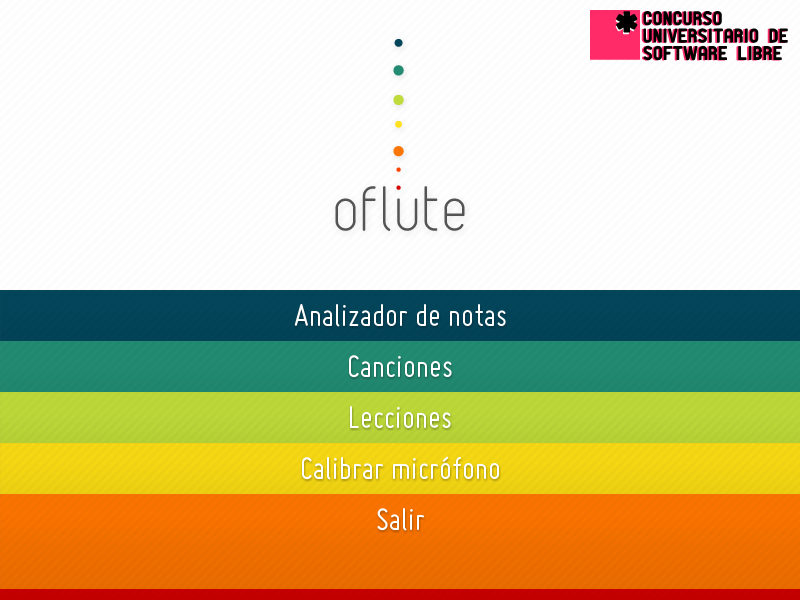
\includegraphics[width=0.8\textwidth]{imagen_menuPrincipal}
%   \caption{Pantalla del menú principal}
% \end{figure}

% \pagebreak

% \begin{figure}[htp!]
%   \centering
%   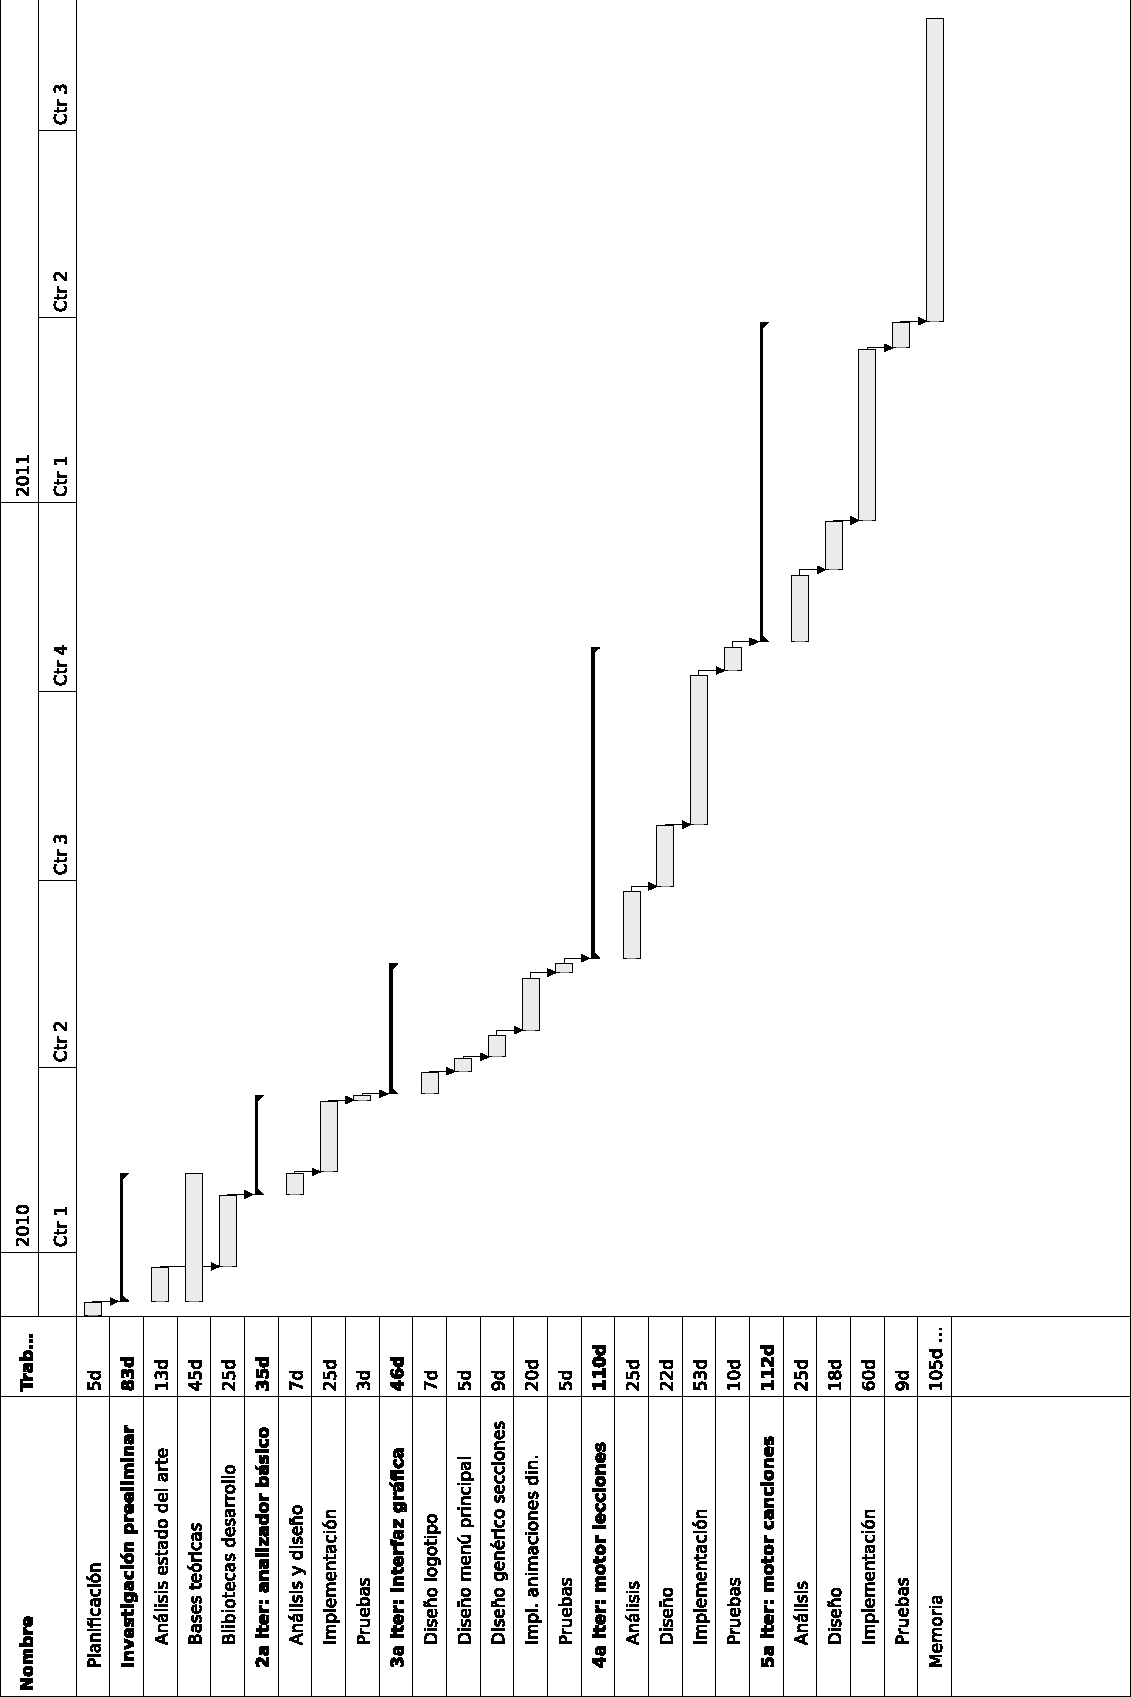
\includegraphics[width=0.95\textwidth]{imagen_diagrama_gantt}
%   \caption{Diagrama Gantt de iteraciones}
%   \label{fig:gantt}
% \end{figure}

% \pagebreak

% \subsection{Análisis de notas}
% Permite a los usuarios comprobar, de manera individual y pausada, que la
% interpretación de cada una de las notas en la flauta es correcta. Para ello, se
% presenta un pequeño analizador que responderá al sonido emitido por el usuario
% con la flauta mostrando la nota tocada en pantalla.

% \begin{figure}[h!]
%   \centering
%   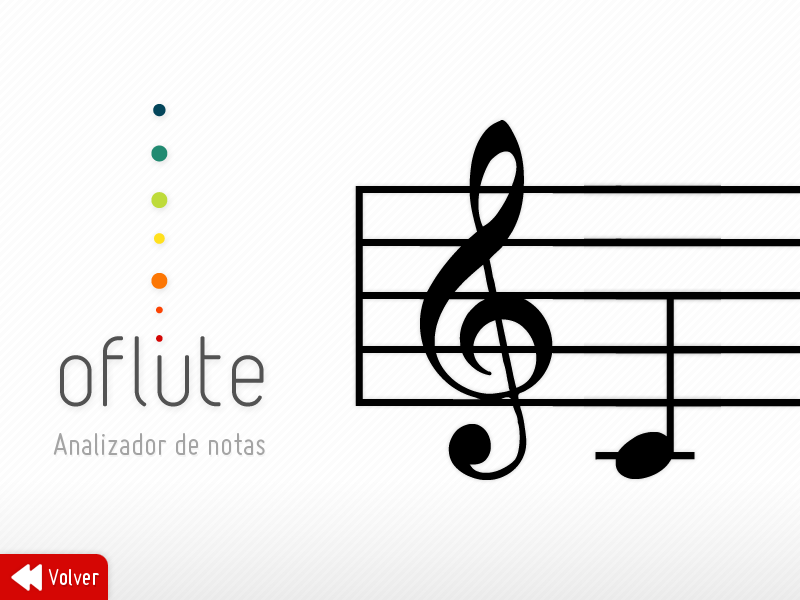
\includegraphics[width=0.8\textwidth]{imagen_seccionAnalizador}
%   \caption{Pantalla del analizador de notas}
% \end{figure}

% \subsection{Motor de canciones}
% Mediante este sistema, el usuario tendrá la oportunidad de interpretar canciones
% completas a la vez que el computador analiza la eficacia del jugador,
% otorgándole una puntuación en tiempo real. Además, el motor de canciones es
% fácilmente expansible mediante ficheros de definición de canciones.

% \subsection{Motor de lecciones}
% Este sistema ofrece al usuario una serie de lecciones multimedia, con las que
% podrá aprender sobre diferentes aspectos de la música en general y la flauta en
% particular. Las lecciones cuentan con imágenes, texto y animaciones, que harán
% que el aprendizaje sea entretenido y ameno. También es posible añadir nuevas
% lecciones al sistema de forma sencilla.

% \begin{figure}[h!]
%   \centering
%   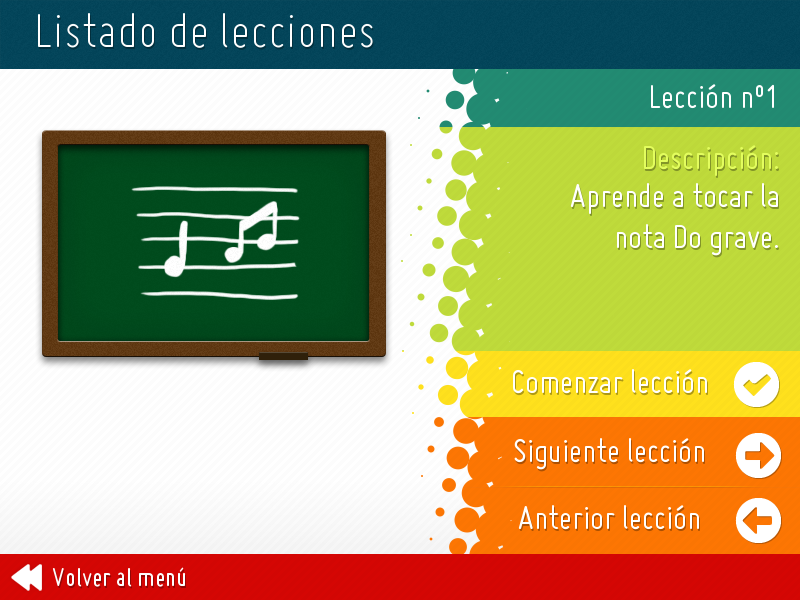
\includegraphics[width=0.8\textwidth]{imagen_seccionLecciones1}
%   \caption{Pantalla del menú de selección de lecciones}
% \end{figure}

% \subsection{Calibración del micrófono}
% \textbf{oFlute} ofrece la posibilidad de calibrar el micrófono, de forma que el
% sistema se adapte al ruido ambiental y el análisis del sonido capturado sea lo
% más exacto posible

% \section{Implementación}
% Durante el desarrollo del proyecto surgieron numerosas cuestiones y decisiones
% de implementación. A continuación se presenta una selección de las que más
% interés han generado. En la memoria del proyecto se desarrollan en mayor
% extensión.

% \subsection{Implementación del analizador básico}
% La creación del analizador básico de notas era crucial para el buen transcurso
% del resto del proyecto, por lo que fue uno de los objetivos que antes se
% abordaron. El desarrollo se dividió en dos partes. Por un lado, había que
% iniciar la captura de audio, lanzando el subsistema de sonido y empezando a
% capturar datos. Por otro lado, se tenía que hacer el análisis de los datos
% leídos para determinar qué nota se estaba tocando.

% La gestión del subsistema de audio se hizo mediante la \textit{Simple API} de
% PulseAudio, la biblioteca de audio que se empleó en oFlute. Se utilizó para la
% configuración y creación de un flujo de audio de entrada que permitiera captar,
% muestrear y samplear el sonido del micrófono, ofreciéndolo en forma de datos en
% punto flotante en un búffer.

% El siguiente paso fue el análisis del audio capturado. Para ello, utilizamos la
% Transformada Rápida de Fourier mediante su implementación en la biblioteca
% KissFFT. De forma iterativa, se iba analizando el búffer de sonido cada vez que
% éste se llenaba, dando lugar a una aproximación de la frecuencia fundamental
% capturada y, por ende, la nota que se estaba interpretando con la flauta.

% Una vez implementado y probado el sistema, se dió por bueno el analizador y se
% siguió construyendo el resto de la aplicación

% \subsection{Carga y uso de fuentes TrueType en Gosu}
% La biblioteca principal utilizada en la implementación del proyecto es Gosu, una
% librería de desarrollo de videojuegos 2D, multi-plataforma y con numerosas
% características. Desafortunadamente, no era posible utilizar fuentes TrueType
% cuando se utilizaba la biblioteca en GNU/Linux.

% Utilizando los conocimientos de otra popular biblioteca, SDL, se consiguió
% implementar un sistema para cargar y usar fuentes TrueType en Gosu de forma
% eficiente. Esta implementación finalmente acabó formando parte oficial de la
% biblioteca Gosu.

% \subsection{Animaciones dinámicas}
% Una de las decisiones iniciales de diseño fue la de hacer la interfaz gráfica de
% usuario lo más atractiva posible, intentando utilizar gráficos amigables y, en
% la medida de lo posible, animaciones y efectos dinámicos.

% Con esto, se tornaba necesario crear un sistema de animaciones lo más versátil
% posible, de forma que dotar a los elementos de la interfaz de movimiento fuera
% un proceso sencillo. 

% Para satisfacer este objetivo se ideó una serie de clases de animación que
% permiten animar las propiedades de los objetos de manera muy sencilla. Mediante
% el uso de las ecuaciones de animación de Robert Penner, el sistema creado cuenta
% con un gran número de opciones y diferentes formas de movimiento, según el tipo
% de función utilizada para calcular los valores: cuadrático, cúbico, etcétera.

% Gracias a este sistema, la interfaz de usuario de oFlute cuenta con un gran
% dinamismo y vistosidad.

% \subsection{Gestión de estados}
% La gestión de estados es uno de los retos principales a la hora de desarrollar
% un videojuego. Es necesario contar un sistema de gestión de estados robusto, que
% permita pasar de un estado a otro de forma sencilla, sin errores, y manteniendo
% información entre transiciones si fuera necesario.

% En el caso de oFlute, se creó un gestor de estados que permitió modularizar
% fácilmente el programa, haciendo una clara división entre secciones y
% facilitando la transición entre ellas. Además, mediante pruebas exhaustivas y el
% uso de herramientas de depuración, el gestor está implementado de forma que la
% carga y descarga de estados sea limpia y sin errores, evitando fugas de memoria.

% \subsection{Internacionalización}
% Durante el desarrolllo del proyecto surgió la necesidad de preparar el proyecto
% para su traducción. Inicialmente se optó por utilizar un sistema propio de
% traducción, basado en un script en Python y en una pequeña clase que generaba un
% diccionario según el idioma elegido. Sin embargo, esta opción resultó
% ineficiente y, sobre todo, alejada del resto de soluciones estándar a la hora de
% traducción de proyectos. 

% Por ello, se decidió investigar sobre las tecnologías de traducción más
% utilizadas en el panorama del software libre, y finalmente se optó por
% \textbf{GNU Gettext}~\cite{refgettext}. Para afianzar los conocimientos y
% facilitar el aprendizaje a otros desarrolladores, se editó un conciso manual
% sobre internacionalización de proyectos, presente como apéndice en la memoria del proyecto fin de



% \section{Conclusiones y difusión}
% Durante el transcurso del desarrollo de oFlute, y sobre todo al término del
% mismo, se han obtenido unas conclusiones y unos resultados, tanto de forma
% personal como para con la comunidad, que se resumen en esta sección y se tratan
% más en profundidad en el capítulo dedicado a tal efecto en la memoria principal.

% \subsection{Objetivos}
% Al término del desarrollo del proyecto, el proyecto ha completado todos los
% objetivos a cumplir, detallados en el planteamiento inicial. En particular:

% \begin{itemize}
% \item Se llevó a cabo la creación del módulo de análisis de sonido, consiguiendo
%   una efectividad en la detección de las notas muy alta.
% \item Se hizo uso del módulo en una sección de análisis de notas y en el propio
%   juego de interpretación de canciones, con resultados muy satisfactorios y
%   funcionamiento correcto.
% \item Además, el sistema de lecciones planteado se llevó a cabo correctamente,
%   consiguiendo un motor dinámico bastante potente y fácilmente ampliable, con
%   opción a añadir nuevas lecciones al sistema.
% \item Finalmente, todos los objetivos se llevaron a cabo respetando la premisa
%   de mantener una interfaz de usuario amigable y fluida, agradable a la vista y
%   sencilla de usar.
% \end{itemize}

% \subsection{Posibles mejoras}
% Hay un gran número de posibles mejoras y extensiones de la funcionalidad de
% oFlute, en unos casos descubiertas de forma personal y en otros casos aportadas
% por terceras personas. Algunas de las más interesantes son las siguientes:
% \begin{itemize}
% \item Extensión del sistema de lecciones para permitir lecciones de varios
%   pasos, así como integrar las lecciones con el analizador de audio para
%   comprobar los conocimientos in-situ.
% \item Mejora de la jugabilidad del sistema de canciones, añadiendo bonus y
%   puntos extra.
% \item Intentar extender el sistema a otros instrumentos o a la voz humana.
% \item Portar el videojuego a la plataforma Windows.
% \end{itemize}

% \subsection{Conclusiones personales}

% oFlute ha sido el proyecto más longevo al que me he enfrentado hasta ahora. A
% pesar de tener conciencia de la envergadura del mismo desde el principio, el
% tiempo para completarlo ha superado todas mis expectativas, sobre todo en lo que
% a documentación se refiere. 

% Gracias a oFlute he aprendido las técnicas básicas de la programación de audio,
% sobre todo en la parte técnica más que teórica. Es esta parte teórica, sobre
% todo la de análisis, la que me gustaría reforzar en un futuro, ahora que cuento
% con las bases para conseguirlo. Los videojuegos relacionados con el audio
% son un nicho aún poco explorado y que puede dar muchas satisfacciones, sobre
% todo cuando el producto se orienta a un público joven.

% Por otro lado, oFlute también me ha ayudado a aprender a usar bastantes
% tecnologías auxiliares, en algunos casos meras herramientas que han facilitado
% el trabajo y, en otros casos, elementos que resultaron ser de inestimable ayuda
% e imprescindible uso al término del proyecto.

% Una de estas tecnologías es \textbf{Boost}~\cite{boost}, un conjunto de
% bibliotecas para C++ que amplían en gran medida la biblioteca estándar del
% lenguaje. Un amplio número de componentes de Boost formarán parte del nuevo
% estándar C++0x, por lo que me ha servido para ponerme al día en las novedades
% que están por llegar.

% Al tratarse de la principal biblioteca utilizada durante el desarrollo, oFlute
% me ha provisto de un profundo conocimiento de \textbf{Gosu}~\cite{gosu},
% permitiéndome implementar videojuegos con mucha más fluidez y labrándome un
% pequeño \textit{framework} personal que utilizar de base en próximos
% proyectos. 

% Otra de las tecnologías que he aprendido ha sido \textbf{GNU Gettext}, que ha
% servido para internacionalizar el proyecto. Aunque inicialmente se pensó en
% utilizar una solución propia para la internacionalización el proyecto,
% posteriormente se decidió usar esta tecnología, ampliamente conocida y
% utilizada.

% \subsection{Difusión}

% \subsubsection{Conocimiento generado}

% Además de servir como recurso para el correcto transcurso del proyecto, los
% conocimientos adquiridos me permitieron, en numerosos casos, generar
% documentación adicional e impartir talleres relacionados las tecnologías
% previamente mencionadas.

% En cuanto a Boost, se llevó a cabo un taller durante los \textit{Cursos de
%   Verano de la OSLUCA}~\cite{cursosverano}, en el que se explicaron las partes
% más importantes de esta colección de bibliotecas, con numerosos ejemplos de
% muchas de ellas. Toda la documentación es libre~\cite{materialesCursoBoost}.

% Por otro lado, impartí un taller~\cite{tallergosu} sobre la biblioteca Gosu en
% colaboración con la ADVUCA~\cite{advuca}, cuya afluencia superó las 50
% personas. Los materiales pueden descargarse
% libremente~\cite{tallergosumateriales}.

% Por último, tras la aplicación de GNU Gettext en oFlute, escribí una guía
% concisa sobre traducción de proyectos con esta herramienta, que se puede
% encontrar en uno de los apéndices de la memoria, así como de forma online en la
% url \url{http://hdl.handle.net/10498/10772}.


% \subsubsection{Freegemas}

% Uno de los proyectos \textit{``hijos''} de oFlute ha sido
% \textbf{Freegemas}~\cite{freegemas}, un clon libre del popular juego tipo puzzle
% \textit{Bejeweled}. Freegemas es multiplataforma, funciona tanto en GNU/Linux
% como en Windows, y además forma parte oficial de Guadalinex~\cite{guadalinex},
% por lo que es posible encontrarlo en los repositorios oficiales.

% Además, Freegemas sirvió como base para una serie de tres artículos que
% publiqué, junto al director del presente PFC, en la revista Linux
% Magazine~\cite{linuxmagazine} sobre desarrollo de videojuegos en C++. Es posible
% encontrar estos artículos en el archivo de la
% revista~\cite{refarticulo1}~\cite{refarticulo2}~\cite{refarticulo3} bajo una
% licencia Creative Commons.

% \subsubsection{IV Concurso Universitario de Software Libre}

% Por otro lado, gracias a oFlute tuve la oportunidad de participar en el IV
% Concurso Universitario de Software Libre~\cite{cusl}. En el transcurso del
% concurso formé parte de una comunidad muy unida, en la que reinó el apoyo y la
% ayuda entre los concursantes. La final del concurso se celebró en la Escuela
% Superior de Ingeniería de Cádiz, en la que oFlute obtuvo una mención
% especial~\cite{cusl2}.

% Previa a la final nacional tuvo lugar la fase local del concurso, en el que el
% proyecto también recibió un accésit al mejor proyecto de
% innovación~\cite{cusllocal}.

% \bibliographystyle{hispa-annote}
% \bibliography{bibliografia}

\end{document}
